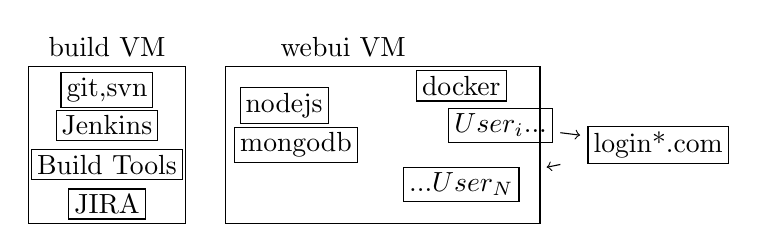
\begin{tikzpicture}

\tikzstyle{mynodestyle} = [draw,outer sep=0,inner sep=1,minimum size=10]

\draw  (0.0,-0.0) rectangle (2.0,-2.0); \node at (1.0,0.25) {build VM};
\draw  (2.5,-0.0) rectangle (6.5,-2.0); \node at (4.0,0.25) {webui VM};

\node [draw,outer sep=10,inner sep=2,minimum size=10] at (1.0,-0.3) {git,svn};

\node [draw,outer sep=10,inner sep=2,minimum size=10] at (1.0,-0.75) {Jenkins};
\node [draw,outer sep=10,inner sep=2,minimum size=10] at (1.0,-1.25) {Build Tools};
\node [draw,outer sep=10,inner sep=2,minimum size=10] at (1.0,-1.75) {JIRA};

\node [draw,outer sep=10,inner sep=2,minimum size=10] at (3.25,-0.5) {nodejs};
\node [draw,outer sep=10,inner sep=2,minimum size=10] at (3.4,-1.0) {mongodb};

\node [draw,outer sep=10,inner sep=2,minimum size=10] at (5.5,-0.25) {docker};

\node [draw,outer sep=10,inner sep=2,minimum size=10] (v2) at (6.0,-0.75) {$User_i$...};
\node [draw,outer sep=10,inner sep=2,minimum size=10] (v3) at (5.5,-1.5) {...$User_N$};

\node [draw,outer sep=10,inner sep=2,minimum size=10] (v1) at (8,-1) {login*.com};




\draw [->] (v1) edge (v2);
\draw [->] (v1) edge (v3);
\end{tikzpicture}